\documentclass[12pt, letterpaper]{article}

\setlength{\topmargin}{-1.75cm} \setlength{\textheight}{22.5cm}
\setlength{\oddsidemargin}{0.25cm}
\setlength{\evensidemargin}{0.25cm} \setlength{\textwidth}{17.2cm}

\usepackage{amssymb}
\usepackage{graphicx}
\usepackage{palatino, url, multicol} % for multiple columns
\usepackage{pictex}
%% in the .pictex output of xfig, there is command \colo
%% however the old version of pictex may not define this
%% so we define color here as empty
\def \color#1]#2{}

\newcommand{\courseTitle}
{
 CS5384 Logic for Computer
Scientists }

\newcommand{\projecttitle} {
  Satisfiability test of clauses and its application
}

\begin{document}
%% \noindent test \hfill test
\title{{\bf Project.} \projecttitle}
\date{} 
 \maketitle
\thispagestyle{myheadings} \markright{CS5384 Logic for Computer
Scientists by Y Zhang, TTU, Fall 2022}

\section*{Team}
1) Lohith Bhargav Doppalapudi, R11786637 \\
   \\
2) Thulasi Priya Nallapothula,    R11797226 \\
   \\
3) Sri Ram Koppaku,     R11842335\\
   \\ \\
\textbf{Intro}:\\
The N-queens problem is about placing n-chess queens on an n*n chessboard so that no two queens are positioned in same vertical, horizantal, and diagonal. we represent the n*n chess board as matrix. Using Back Tracking the problem is solved.\\
\\
\textbf{Possibilities}:\\
The two possibilities in solving NQueens problem are HillClimbing, Backtrack Algorithim\\
\\
\textbf{HillClimbing Algorithm}: It is an iterative algorithm that starts with an arbitary solution to a problem, then attempts to find a better solution by incrementally changing a single element of the solution. This is a local search algorithm. The algorithm does not maintain a search tree, so the data structure for the current node need only record the state and the value of the objective function.\\
\\
\textbf{Backtrack Algorithm}: If a queen is under attack at all the positions in a row, coloum, and diagonal we backtrack and change the position of the queen placed prior to the current position. We repeat this process of placing a queen and backtracking until all the N queens are placed successfully.\\
\\ \textbf{Pseudocode}:\\
\\def minimumOne(List):\\
\indent   initialize a variable\\
\indent   loop over the list\\
\indent  \indent	checking for minimum one variable in list for true\\
\indent    appending ‘0’ for each row\\
\\def maximumOne(List) :\\
\indent    initialize a variable\\
\indent    loop over the list\\
\indent \indent	loop over the list’s list\\
\indent \indent	 checking for maximum one variable in list for true\\
\\def varmap(row,column,size):\\
\indent    to return the grid\\
\\def preciselyOne(List):\\
\indent    initialize a variable\\
\indent    variable is appended with minimumOne(list) return value\\
\indent    variable is appended with maximumOne(list) return value\\
\\loop over row in (0, N): \\
\indent \indent	initialize a list  \\
\indent \indent    	loop over col in (0, N):\\
\indent        appending position to check to have precisely 1 queen per row\\
\\loop over col in (0, N): \\
\indent \indent	initialize a list  \\
\indent \indent    	loop over row in (0, N):\\
\indent        appending position to check to have precisely 1 queen per column\\
\\loop over col in (0, N): \\
\indent \indent	initialize a list  \\
\indent \indent    	loop over x in (0, N):\\
\indent        appending position to check to have precisely 1 queen per column\\
\\loop over row in (N-1, -1, -1): \\
\indent \indent	initialize a list  \\
\indent \indent    	loop over x in (0, N-row):\\
\indent        appending position to list for maximum of 1 queen per -ve diagonal from left\\
\\loop over col in (1, N): \\
\indent \indent	initialize a list  \\
\indent \indent    	loop over x in (0, N-col):\\
\indent        appending position to list for maximum of 1 queen per -ve diagonal from top\\
\\loop over row in (N-1, -1, -1): \\
\indent \indent	initialize a list  \\
\indent \indent    	loop over x in row(0, N-row):\\
\indent        appending position to list for maximum of 1 queen per +ve diagonal from right\\
\\loop over col in (N-2, -1, -1): \\
\indent \indent	initialize a list  \\
\indent \indent    	loop over x in col(0, col+1):\\
\indent        appending position to list for maximum of 1 queen per +ve diagonal from top\\
\\creating a cnf file to store in dimacs CNF format\\
\\appending the p cnf no.of positions, no.of variables and clauses\\
\\ \textbf{Files in RAR}:\\
Nqueens.py which generates the CNF file with DIMACS format \\
Run.sh is a scripting language commands file that contains computer program to be run by Unix shell \\
\\ \textbf{How to Execute}:\\
Run the script code (run.sh) by sh run.sh command\\
It will prompt for the nqueens input of matrix\\
\\ \textbf{Output}: \\
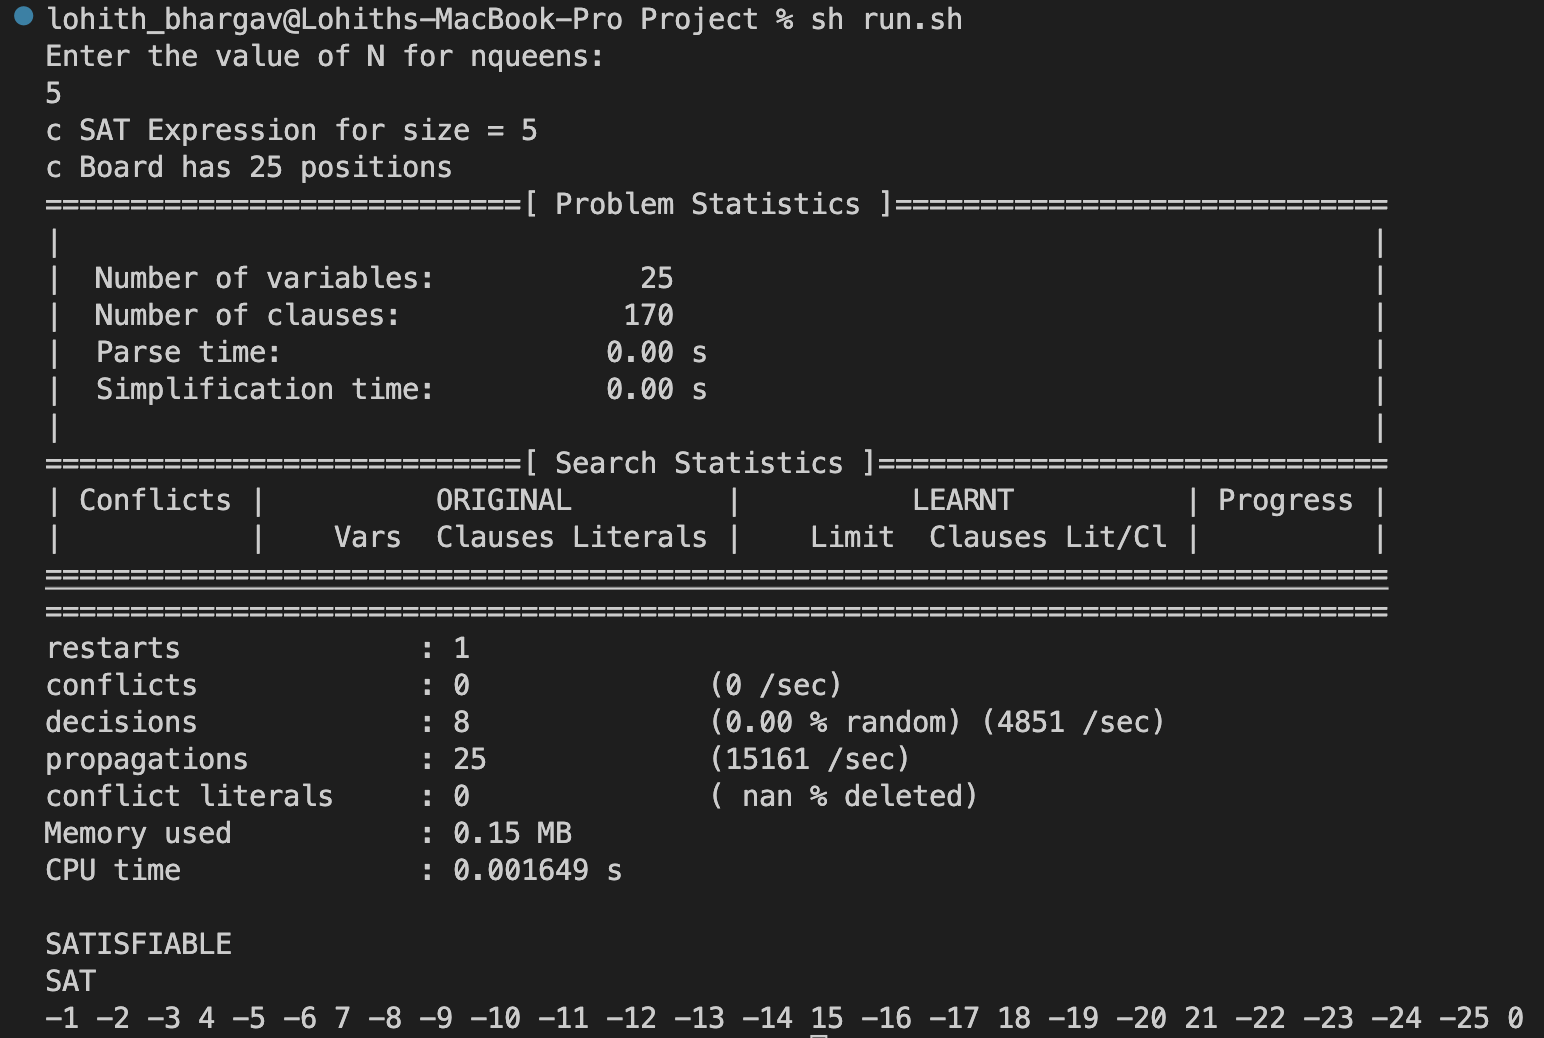
\includegraphics[width=0.8\textwidth]{Output.png}

\end{document}
